% Options for packages loaded elsewhere
\PassOptionsToPackage{unicode}{hyperref}
\PassOptionsToPackage{hyphens}{url}
\PassOptionsToPackage{dvipsnames,svgnames,x11names}{xcolor}
\documentclass[
  10pt,
  ignorenonframetext,
  serif,
  aspectratio=169]{beamer}
\newif\ifbibliography
\usepackage{pgfpages}
\setbeamertemplate{caption}[numbered]
\setbeamertemplate{caption label separator}{: }
\setbeamercolor{caption name}{fg=normal text.fg}
\beamertemplatenavigationsymbolsempty
% remove section numbering
\setbeamertemplate{part page}{
  \centering
  \begin{beamercolorbox}[sep=16pt,center]{part title}
    \usebeamerfont{part title}\insertpart\par
  \end{beamercolorbox}
}
\setbeamertemplate{section page}{
  \centering
  \begin{beamercolorbox}[sep=12pt,center]{section title}
    \usebeamerfont{section title}\insertsection\par
  \end{beamercolorbox}
}
\setbeamertemplate{subsection page}{
  \centering
  \begin{beamercolorbox}[sep=8pt,center]{subsection title}
    \usebeamerfont{subsection title}\insertsubsection\par
  \end{beamercolorbox}
}
% Prevent slide breaks in the middle of a paragraph
\widowpenalties 1 10000
\raggedbottom
\AtBeginPart{
  \frame{\partpage}
}
\AtBeginSection{
  \ifbibliography
  \else
    \frame{\sectionpage}
  \fi
}
\AtBeginSubsection{
  \frame{\subsectionpage}
}
\usepackage{iftex}
\ifPDFTeX
  \usepackage[T1]{fontenc}
  \usepackage[utf8]{inputenc}
  \usepackage{textcomp} % provide euro and other symbols
\else % if luatex or xetex
  \usepackage{unicode-math} % this also loads fontspec
  \defaultfontfeatures{Scale=MatchLowercase}
  \defaultfontfeatures[\rmfamily]{Ligatures=TeX,Scale=1}
\fi
\usepackage{lmodern}
\ifPDFTeX\else
  % xetex/luatex font selection
\fi
% Use upquote if available, for straight quotes in verbatim environments
\IfFileExists{upquote.sty}{\usepackage{upquote}}{}
\IfFileExists{microtype.sty}{% use microtype if available
  \usepackage[]{microtype}
  \UseMicrotypeSet[protrusion]{basicmath} % disable protrusion for tt fonts
}{}
\makeatletter
\@ifundefined{KOMAClassName}{% if non-KOMA class
  \IfFileExists{parskip.sty}{%
    \usepackage{parskip}
  }{% else
    \setlength{\parindent}{0pt}
    \setlength{\parskip}{6pt plus 2pt minus 1pt}}
}{% if KOMA class
  \KOMAoptions{parskip=half}}
\makeatother
\usepackage{color}
\usepackage{fancyvrb}
\newcommand{\VerbBar}{|}
\newcommand{\VERB}{\Verb[commandchars=\\\{\}]}
\DefineVerbatimEnvironment{Highlighting}{Verbatim}{commandchars=\\\{\}}
% Add ',fontsize=\small' for more characters per line
\newenvironment{Shaded}{}{}
\newcommand{\AlertTok}[1]{\textcolor[rgb]{1.00,0.00,0.00}{\textbf{#1}}}
\newcommand{\AnnotationTok}[1]{\textcolor[rgb]{0.38,0.63,0.69}{\textbf{\textit{#1}}}}
\newcommand{\AttributeTok}[1]{\textcolor[rgb]{0.49,0.56,0.16}{#1}}
\newcommand{\BaseNTok}[1]{\textcolor[rgb]{0.25,0.63,0.44}{#1}}
\newcommand{\BuiltInTok}[1]{\textcolor[rgb]{0.00,0.50,0.00}{#1}}
\newcommand{\CharTok}[1]{\textcolor[rgb]{0.25,0.44,0.63}{#1}}
\newcommand{\CommentTok}[1]{\textcolor[rgb]{0.38,0.63,0.69}{\textit{#1}}}
\newcommand{\CommentVarTok}[1]{\textcolor[rgb]{0.38,0.63,0.69}{\textbf{\textit{#1}}}}
\newcommand{\ConstantTok}[1]{\textcolor[rgb]{0.53,0.00,0.00}{#1}}
\newcommand{\ControlFlowTok}[1]{\textcolor[rgb]{0.00,0.44,0.13}{\textbf{#1}}}
\newcommand{\DataTypeTok}[1]{\textcolor[rgb]{0.56,0.13,0.00}{#1}}
\newcommand{\DecValTok}[1]{\textcolor[rgb]{0.25,0.63,0.44}{#1}}
\newcommand{\DocumentationTok}[1]{\textcolor[rgb]{0.73,0.13,0.13}{\textit{#1}}}
\newcommand{\ErrorTok}[1]{\textcolor[rgb]{1.00,0.00,0.00}{\textbf{#1}}}
\newcommand{\ExtensionTok}[1]{#1}
\newcommand{\FloatTok}[1]{\textcolor[rgb]{0.25,0.63,0.44}{#1}}
\newcommand{\FunctionTok}[1]{\textcolor[rgb]{0.02,0.16,0.49}{#1}}
\newcommand{\ImportTok}[1]{\textcolor[rgb]{0.00,0.50,0.00}{\textbf{#1}}}
\newcommand{\InformationTok}[1]{\textcolor[rgb]{0.38,0.63,0.69}{\textbf{\textit{#1}}}}
\newcommand{\KeywordTok}[1]{\textcolor[rgb]{0.00,0.44,0.13}{\textbf{#1}}}
\newcommand{\NormalTok}[1]{#1}
\newcommand{\OperatorTok}[1]{\textcolor[rgb]{0.40,0.40,0.40}{#1}}
\newcommand{\OtherTok}[1]{\textcolor[rgb]{0.00,0.44,0.13}{#1}}
\newcommand{\PreprocessorTok}[1]{\textcolor[rgb]{0.74,0.48,0.00}{#1}}
\newcommand{\RegionMarkerTok}[1]{#1}
\newcommand{\SpecialCharTok}[1]{\textcolor[rgb]{0.25,0.44,0.63}{#1}}
\newcommand{\SpecialStringTok}[1]{\textcolor[rgb]{0.73,0.40,0.53}{#1}}
\newcommand{\StringTok}[1]{\textcolor[rgb]{0.25,0.44,0.63}{#1}}
\newcommand{\VariableTok}[1]{\textcolor[rgb]{0.10,0.09,0.49}{#1}}
\newcommand{\VerbatimStringTok}[1]{\textcolor[rgb]{0.25,0.44,0.63}{#1}}
\newcommand{\WarningTok}[1]{\textcolor[rgb]{0.38,0.63,0.69}{\textbf{\textit{#1}}}}
\usepackage{longtable,booktabs,array}
\usepackage{caption}
\captionsetup[table]{skip=6pt}
\newcounter{none} % for unnumbered tables
\usepackage{calc} % for calculating minipage widths
\usepackage{caption}
% Make caption package work with longtable
\makeatletter
\def\fnum@table{\tablename~\thetable}
\makeatother
\usepackage{graphicx}
\makeatletter
\newsavebox\pandoc@box
\newcommand*\pandocbounded[1]{% scales image to fit in text height/width
  \sbox\pandoc@box{#1}%
  \Gscale@div\@tempa{\textheight}{\dimexpr\ht\pandoc@box+\dp\pandoc@box\relax}%
  \Gscale@div\@tempb{\linewidth}{\wd\pandoc@box}%
  \ifdim\@tempb\p@<\@tempa\p@\let\@tempa\@tempb\fi% select the smaller of both
  \ifdim\@tempa\p@<\p@\scalebox{\@tempa}{\usebox\pandoc@box}%
  \else\usebox{\pandoc@box}%
  \fi%
}
% Set default figure placement to htbp
\def\fps@figure{htbp}
\makeatother
\setlength{\emergencystretch}{3em} % prevent overfull lines
\providecommand{\tightlist}{%
  \setlength{\itemsep}{0pt}\setlength{\parskip}{0pt}}
% -*- coding: utf-8 -*-
% Preamble for md-to-tex-slides.md (included via `include-in-header` in
% md-to-tex-beamer.yaml).  It lives in a file because pandoc parses
% `header-includes` values as Markdown, which mangles raw LaTeX such as
% fontspec's `[RawFeature={fallback=...}]`.
\usepackage{fontspec}
\directlua{luaotfload.add_fallback("emojifb", {"Segoe UI Emoji:mode=harf"})}
\setsansfont{Latin Modern Sans}[RawFeature={fallback=emojifb}]
\setmainfont{Latin Modern Roman}[RawFeature={fallback=emojifb}]
\setmonofont{Latin Modern Mono}[RawFeature={fallback=emojifb},Scale=0.86]

\usepackage{amsmath,amssymb}
\usepackage{xcolor}
\definecolor{nordred}{HTML}{BF616A}
\definecolor{nordblue}{HTML}{5E81AC}
\definecolor{nordgreen}{HTML}{A3BE8C}
\definecolor{nordyellow}{HTML}{EBCB8B}
\definecolor{nordpurple}{HTML}{B48EAD}
\definecolor{norddark}{HTML}{2E3440}
\definecolor{nordlight}{HTML}{ECEFF4}

\usepackage{pgf,tikz}
\usetikzlibrary{arrows.meta,positioning,shapes.geometric,calc,fit,backgrounds}
\tikzset{
  nb/.style={draw, rounded corners, align=center, font=\scriptsize,
             inner sep=4pt, minimum height=7mm},
  nblue/.style={nb, fill=blue!12,  draw=nordblue,  line width=1pt},
  nyellow/.style={nb, fill=yellow!35, draw=orange!80!black, line width=1pt},
  npurple/.style={nb, fill=violet!14, draw=nordpurple, line width=1pt},
  nred/.style={nb, fill=red!12, draw=nordred, line width=1.5pt},
  ngreen/.style={nb, fill=green!16, draw=green!45!black, line width=1pt},
  npink/.style={nb, fill=magenta!10, draw=magenta!70!black, line width=1pt},
  ar/.style={-{Stealth[length=2mm]}, draw=black!55, line width=0.8pt},
}

\usepackage{listings}
\lstset{
  basicstyle=\ttfamily\scriptsize,
  breaklines=true,
  showstringspaces=false,
  columns=fullflexible,
  frame=single,
  rulecolor=\color{black!20},
}

\usetheme{Frankfurt}
\setbeamertemplate{navigation symbols}{}
\setbeamercolor{structure}{fg=nordblue}
\setbeamercolor{frametitle}{fg=norddark,bg=nordlight}
\setbeamercolor{math text}{fg=nordblue}
\setbeamercovered{transparent}

\newcommand{\columnsbegin}{\begin{columns}}
\newcommand{\columnsend}{\end{columns}}
\newcommand{\col}[1]{\column{#1}}
\usepackage{bookmark}
\IfFileExists{xurl.sty}{\usepackage{xurl}}{} % add URL line breaks if available
\urlstyle{same}
% fallback for those not using the hyperref driver hyperxmp:
\makeatletter
\@ifundefined{xmpquote}{\newcommand{\xmpquote}[1]{#1}}{}
\makeatother
\hypersetup{
  pdftitle={From Markdown to TeX},
  pdfauthor={Wai-Shing Luk},
  colorlinks=true,
  linkcolor={Maroon},
  filecolor={Maroon},
  citecolor={Blue},
  urlcolor={Blue},
  pdfcreator={LaTeX via pandoc}}

\title{\texorpdfstring{From Markdown to TeX}{From Markdown to TeX}}
\subtitle{\texorpdfstring{A Pandoc paper pipeline --- and the traps that
break it}{A Pandoc paper pipeline --- and the traps that break it}}
\author{\texorpdfstring{Wai-Shing Luk}{Wai-Shing Luk}}
\date{\today}
\institute{Fudan University}

\begin{document}
\frame{\titlepage}

\section{Agenda}\label{agenda}

\begin{frame}[fragile]{📋 Agenda}
\protect\phantomsection\label{agenda-1}
\begin{columns}[T]
\begin{column}{0.47\linewidth}
\textbf{🔧 Part 1 --- The Pipeline} Why Markdown, not raw TeX? · pandoc
+ crossref + citeproc · anatomy of a source

\textbf{⚙️ Part 2 --- The Build} the command, flag by flag · one entry
point: \texttt{make}
\end{column}

\begin{column}{0.47\linewidth}
\textbf{🐛 Part 3 --- War Stories} emoji \& Unicode · SVG figures ·
headings \& cleveref · offline citations

\textbf{🎯 Part 4 --- Takeaways} a reproducibility checklist
\end{column}
\end{columns}
\end{frame}

\section{The Pipeline}\label{the-pipeline}

\begin{frame}{🤔 Why Write Markdown, Not Raw TeX?}
\protect\phantomsection\label{why-write-markdown-not-raw-tex}
\begin{columns}[T]
\begin{column}{0.47\linewidth}
\textbf{Markdown wins ✅}

\begin{itemize}
\tightlist
\item
  Readable plain text 📖
\item
  Diffs are \emph{semantic}, not macro noise 🔍
\item
  Math stays LaTeX 📐
\item
  One source → PDF, HTML, slides 🎯
\end{itemize}
\end{column}

\begin{column}{0.47\linewidth}
\textbf{But TeX wins at 🏆}

\begin{itemize}
\tightlist
\item
  Precise typesetting 📕
\item
  Journal classes 🏛️
\item
  Cross-refs, citations, floats 🔢
\end{itemize}
\end{column}
\end{columns}

\begin{quote}
\textbf{pandoc} is the bridge: Markdown \textbf{in}, TeX \textbf{out},
then a real engine compiles it. 🌉
\end{quote}
\end{frame}

\begin{frame}[fragile]{🏭 The Toolchain}
\protect\phantomsection\label{the-toolchain}
\begin{center}
\begin{tikzpicture}[node distance=9mm and 11mm]
  \node[nblue] (md) {📝 Markdown\\+ YAML};
  \node[nyellow, right=of md] (p) {pandoc};
  \node[npurple, right=of p] (cp) {citeproc};
  \node[nyellow, right=of cp] (x) {crossref};
  \node[npink, below=8mm of x] (t) {📜 TeX};
  \node[ngreen, left=of t] (e) {engine};
  \node[ngreen, left=of e] (pdf) {📕 PDF};
  \node[nblue, above=6mm of p, font=\tiny] (y) {🗂️ latex.yaml};
  \node[npurple, above=6mm of cp, font=\tiny] (b) {📚 *.bib · 🎨 *.csl};
  \draw[ar] (md) -- (p);
  \draw[ar] (p) -- (cp);
  \draw[ar] (cp) -- (x);
  \draw[ar] (x) -- (t);
  \draw[ar] (t) -- (e);
  \draw[ar] (e) -- (pdf);
  \draw[ar] (y) -- (p);
  \draw[ar] (b) -- (cp);
\end{tikzpicture}
\end{center}

\begin{itemize}
\tightlist
\item
  \textbf{citeproc} resolves citations with a \texttt{*.bib} database
  and a \texttt{*.csl} style 📚
\item
  \textbf{pandoc-crossref} resolves labelled headings, figures and
  equations 🏷️
\end{itemize}
\end{frame}

\begin{frame}[fragile]{🧬 Anatomy of a Pandoc-Markdown Paper}
\protect\phantomsection\label{anatomy-of-a-pandoc-markdown-paper}
Everything is plain text --- yet each \texttt{@}-thing is
\textbf{load-bearing}:

{\def\LTcaptype{none} % do not increment counter
\begin{longtable}[]{@{}ll@{}}
\toprule\noalign{}
syntax & meaning \\
\midrule\noalign{}
\endhead
YAML front matter & metadata: title, author, bibliography 🗂️ \\
\texttt{\#\#\ H\ \{\#sec:foo\}} & a labelled heading 🏷️ \\
\texttt{@sec:foo} & cross-reference → ``§ 2'' 🔗 \\
\texttt{{[}@BGT81{]}} & citation → ``{[}1{]}'' 📚 \\
math delimiters & inline \& display math 📐 \\
\texttt{!{[}alt{]}(fig.svg)} & a figure 🖼️ \\
\bottomrule\noalign{}
\end{longtable}
}

\begin{quote}
⚠️ A typo in any of these becomes a \texttt{??}, a missing reference, or
a hard build error.
\end{quote}
\end{frame}

\begin{frame}[fragile]{🗂️ YAML Front Matter = Document Metadata}
\protect\phantomsection\label{yaml-front-matter-document-metadata}
\begin{Shaded}
\begin{Highlighting}[]
\FunctionTok{title}\KeywordTok{:}\AttributeTok{ }\StringTok{"Ellipsoid Method and the Amazing Oracles"}
\FunctionTok{bibliography}\KeywordTok{:}\AttributeTok{ }\KeywordTok{[}\StringTok{"ellipsoid.bib"}\KeywordTok{,}\AttributeTok{ }\StringTok{"fir{-}ref.bib"}\KeywordTok{]}
\FunctionTok{csl}\KeywordTok{:}\AttributeTok{ }\StringTok{"applied{-}mathematics{-}letters.csl"}
\FunctionTok{abstract}\KeywordTok{: }\CharTok{|}
\NormalTok{  The ellipsoid method is a powerful optimization technique ...}
\end{Highlighting}
\end{Shaded}

\begin{itemize}
\tightlist
\item
  \texttt{title} / \texttt{author} → \texttt{\textbackslash{}title} /
  \texttt{\textbackslash{}author} 📕
\item
  \texttt{bibliography} → which BibTeX files to search 📚
\item
  \texttt{csl} → the \textbf{citation style} 🎨
\item
  extra YAML files add \textbf{class options}: \texttt{latex.yaml},
  \texttt{crossref.yaml} ⚙️
\end{itemize}

\begin{quote}
Metadata is passed as \textbf{positional inputs} \emph{before} the
\texttt{.md}. 🧩
\end{quote}
\end{frame}

\begin{frame}[fragile]{📚 Citations: From \texttt{{[}@key{]}} to
\texttt{{[}1{]}}}
\protect\phantomsection\label{citations-from-key-to-1}
\begin{center}
\begin{tikzpicture}[node distance=10mm and 14mm]
  \node[nblue] (k) {citation\\in source};
  \node[npurple, right=of k] (cp) {citeproc};
  \node[npurple, above=7mm of cp] (db) {📚 ellipsoid.bib};
  \node[npurple, below=7mm of cp] (csl) {🎨 applied-math.csl};
  \node[ngreen, right=of cp] (n) {[1]\\citation};
  \node[ngreen, below=8mm of n] (ref) {📖 References\\auto-generated};
  \draw[ar] (k) -- (cp);
  \draw[ar] (db) -- (cp);
  \draw[ar] (csl) -- (cp);
  \draw[ar] (cp) -- (n);
  \draw[ar] (cp) |- (ref);
\end{tikzpicture}
\end{center}

\begin{itemize}
\tightlist
\item
  \texttt{{[}@key{]}} parenthetical · \texttt{@key} narrative ·
  \texttt{{[}@a;\ @b{]}} multiple ✍️
\item
  Cite only keys in a \textbf{listed} \texttt{.bib} --- otherwise the
  reference silently vanishes 🕳️
\end{itemize}
\end{frame}

\begin{frame}[fragile]{🔗 Cross-References: From \texttt{@sec:label} to
``§ 2''}
\protect\phantomsection\label{cross-references-from-seclabel-to-2}
\begin{center}
\begin{tikzpicture}[node distance=12mm and 20mm]
  \node[nblue] (l) {labelled heading\\\texttt{\{\#sec:cutting\_plane\}}};
  \node[nblue, below=12mm of l] (r) {reference\\\texttt{see @sec:cutting\_plane}};
  \node[nyellow, right=28mm of l] (x) {pandoc-crossref};
  \node[ngreen, right=of x] (out) {see § 2};
  \draw[ar] (l) -- (x);
  \draw[ar] (r) -- (x);
  \draw[ar] (x) -- (out);
\end{tikzpicture}
\end{center}

\begin{itemize}
\tightlist
\item
  label prefixes: \texttt{sec} · \texttt{fig} · \texttt{eq} ·
  \texttt{tbl} · \texttt{lst} 🏷️
\item
  \textbf{the separator is file-specific} ⚠️ --- \texttt{ell-review.md}
  uses \texttt{\_}, \texttt{ell-review2.md} uses \texttt{-}
\item
  a mismatched separator \textbf{silently breaks} the link → \texttt{??}
  🕳️
\end{itemize}
\end{frame}

\begin{frame}[fragile]{📐 Math: LaTeX Syntax, Rendered Twice}
\protect\phantomsection\label{math-latex-syntax-rendered-twice}
Markdown math \textbf{is} LaTeX --- pandoc passes it through, and the
web renders it with KaTeX:

\[
\mathcal{E}(x_c, P) \;=\; \{\, x \mid (x - {\color{nordblue}x_c})^{\top}
  {\color{nordred}P}^{-1} (x - {\color{nordblue}x_c}) \le 1 \,\}
\]

\begin{itemize}
\tightlist
\item
  in the \textbf{PDF} → real TeX, typeset by the LaTeX engine 📕
\item
  in the \textbf{HTML} → KaTeX, rendered in the browser 📐
\end{itemize}

\begin{quote}
⚠️ Keep math \textbf{inside math delimiters}. Bare Unicode (\(\tau\),
\(x^2\)) in running text is what breaks \texttt{pdflatex}.
\end{quote}
\end{frame}

\section{The Build}\label{the-build}

\begin{frame}[fragile]{🛠️ The Command, Flag by Flag}
\protect\phantomsection\label{the-command-flag-by-flag}
\begin{Shaded}
\begin{Highlighting}[]
\ExtensionTok{pandoc} \AttributeTok{{-}F}\NormalTok{ pandoc{-}crossref }\AttributeTok{{-}{-}citeproc} \AttributeTok{{-}s} \AttributeTok{{-}t}\NormalTok{ latex }\AttributeTok{{-}N} \AttributeTok{{-}{-}reference{-}links} \DataTypeTok{\textbackslash{}}
  \AttributeTok{{-}{-}shift{-}heading{-}level{-}by}\OperatorTok{=}\NormalTok{{-}1 }\DataTypeTok{\textbackslash{}}
  \AttributeTok{{-}{-}csl}\OperatorTok{=}\NormalTok{applied{-}mathematics{-}letters.csl }\DataTypeTok{\textbackslash{}}
\NormalTok{  ell{-}review.yaml latex.yaml crossref.yaml ell{-}review.md }\AttributeTok{{-}o}\NormalTok{ ell{-}review.pdf}
\end{Highlighting}
\end{Shaded}

{\def\LTcaptype{none} % do not increment counter
\begin{longtable}[]{@{}ll@{}}
\toprule\noalign{}
flag & what it does \\
\midrule\noalign{}
\endhead
\texttt{-F\ pandoc-crossref} & resolve heading / figure / equation
labels 🏷️ \\
\texttt{-\/-citeproc} & process citations + build References 📚 \\
\texttt{-s\ -t\ latex} & standalone LaTeX 📜 \\
\texttt{-\/-shift-heading-level-by=-1} & \texttt{\#\#} →
\texttt{\textbackslash{}section} 🪜 \\
\texttt{-\/-csl=...} & pick the citation style 🎨 \\
\bottomrule\noalign{}
\end{longtable}
}
\end{frame}

\begin{frame}[fragile]{🧩 \texttt{pandoc-crossref}: \texttt{cref}, or
plain \texttt{ref}?}
\protect\phantomsection\label{pandoc-crossref-cref-or-plain-ref}
\begin{center}
\begin{tikzpicture}[node distance=10mm and 14mm]
  \node[npurple] (cfg) {\texttt{crossref.yaml}\\\texttt{cref} option};
  \node[nblue, above right=6mm and 20mm of cfg] (tt) {\texttt{true} → cleveref};
  \node[nyellow, below right=6mm and 20mm of cfg] (ff) {\texttt{false} → ref + §};
  \node[nred, right=of tt] (bad) {siamltex class: \texttt{??} ❌};
  \node[ngreen, right=of ff] (good) {always works ✅};
  \draw[ar] (cfg) -- (tt);
  \draw[ar] (cfg) -- (ff);
  \draw[ar] (tt) -- (bad);
  \draw[ar] (ff) -- (good);
\end{tikzpicture}
\end{center}

\begin{quote}
Our policy: \textbf{\texttt{cref:\ false}} --- a plain reference plus a
literal \textbf{§} prefix. No cleveref, no \texttt{??}. 🎯
\end{quote}
\end{frame}

\section{War Stories}\label{war-stories}

\begin{frame}[fragile]{☠️ War Story 1: Emoji \& Unicode Break
\texttt{pdflatex}}
\protect\phantomsection\label{war-story-1-emoji-unicode-break-pdflatex}
\begin{itemize}
\tightlist
\item
  one emoji 🪜 →
  \texttt{!\ Unicode\ character\ (U+1FA9C)\ not\ set\ up\ for\ use\ with\ LaTeX}
  ❌
\item
  but also \textbf{bare Unicode math} in running text: \(x^2\), \(\le\),
  \(\tau\), \(\beta_1\), \(\to\) ☠️
\end{itemize}

\[
\text{broken: } \; x^2/4 \qquad \text{good: } \; {\color{nordgreen}\tfrac{x^2}{4} + y^2 \le 1}
\]

\begin{center}
\begin{tikzpicture}[node distance=14mm and 24mm]
  \node[nred] (e) {emoji \& bare Unicode};
  \node[nred, right=of e] (err) {\texttt{pdflatex}: Unicode not set up};
  \node[nyellow, below=10mm of e] (fix) {wrap math in delimiters};
  \node[ngreen, right=of fix] (ok) {builds ✅};
  \draw[ar] (e) -- (err);
  \draw[ar] (fix) -- (ok);
\end{tikzpicture}
\end{center}
\end{frame}

\begin{frame}[fragile]{🐛 War Story 2: \texttt{\textbackslash{}argmax}
Is Not a Command}
\protect\phantomsection\label{war-story-2-argmax-is-not-a-command}
\begin{itemize}
\tightlist
\item
  the source wrote \texttt{\textbackslash{}argmax} --- but neither LaTeX
  nor KaTeX defines it ❌
\item
  result: \texttt{!\ Undefined\ control\ sequence} --- the build stops
  🛑
\end{itemize}

The fix is a \emph{real} operator 🪄

\[
q_{\max} \;=\; {\color{nordgreen}\operatorname*{arg\,max}_{q \in \mathcal{Q}}}\; f_0(x_0, q)
\]

\begin{itemize}
\tightlist
\item
  \texttt{\textbackslash{}operatorname*\{arg\textbackslash{},max\}}
  needs \texttt{amsmath} --- pandoc already loads it ✅
\item
  the \textbf{same bug} hid in the slide source --- fix once, fix
  everywhere 🔁
\end{itemize}
\end{frame}

\begin{frame}[fragile]{🪜 War Story 3: Heading Levels →
\texttt{\textbackslash{}section}}
\protect\phantomsection\label{war-story-3-heading-levels-section}
A formatter demoted \texttt{\#} → \texttt{\#\#}; pandoc then emitted
\textbf{no} \texttt{\textbackslash{}section} at all.

\begin{center}
\begin{tikzpicture}[node distance=12mm and 26mm]
  \node[ngreen] (h1) {level-1 heading};
  \node[ngreen, right=of h1] (s) {\texttt{section}\\numbering 1, 2 ✅};
  \node[nred, below=10mm of h1] (h2) {level-2 heading};
  \node[nred, right=of h2] (ss) {\texttt{subsection}\\numbering 0.1, 0.2 😱};
  \draw[ar] (h1) -- (s);
  \draw[ar] (h2) -- (ss);
\end{tikzpicture}
\end{center}

\begin{itemize}
\tightlist
\item
  before: body headings at \texttt{\#} →
  \texttt{\textbackslash{}section} → ``\textbf{1. Introduction}'' ✅
\item
  after the demotion: every heading became
  \texttt{\textbackslash{}subsection} → ``\textbf{0.1 Introduction}'' 😱
\item
  fix \textbf{without touching the prose}:
  \texttt{-\/-shift-heading-level-by=-1} 🪄
\end{itemize}
\end{frame}

\begin{frame}[fragile]{🖼️ War Story 4: SVG Figures Need a Converter}
\protect\phantomsection\label{war-story-4-svg-figures-need-a-converter}
\begin{center}
\begin{tikzpicture}[node distance=10mm and 16mm]
  \node[nblue] (img) {figure link\\to \texttt{*.svg}};
  \node[nyellow, right=of img] (p) {pandoc → LaTeX};
  \node[ngreen, above right=4mm and 14mm of p] (pdf) {\texttt{svg} → \texttt{pdf}\\\texttt{\textbackslash includegraphics} ✅};
  \node[ngreen, below right=4mm and 14mm of p] (twin) {use the \texttt{*.pdf}\\\texttt{twin} ✅};
  \node[nred, right=14mm of p] (svg) {\texttt{svg} pkg + InkScape\\+ shell-escape ❌};
  \draw[ar] (img) -- (p);
  \draw[ar] (p) -- (pdf);
  \draw[ar] (p) -- (twin);
  \draw[ar] (p) -- (svg);
\end{tikzpicture}
\end{center}

\begin{itemize}
\tightlist
\item
  \texttt{pdflatex} cannot read \texttt{.svg} --- pandoc wants
  \textbf{\texttt{rsvg-convert}} (librsvg) 🏭
\item
  missing it → the LaTeX \texttt{svg} package → needs \textbf{InkScape +
  \texttt{-\/-shell-escape}} ❌
\item
  our shortcut: reference the \textbf{\texttt{.pdf} twin} already
  shipped beside every \texttt{.svg} 🎯
\end{itemize}
\end{frame}

\begin{frame}[fragile]{😱 War Story 5: \texttt{rsvg-convert} Drops Text}
\protect\phantomsection\label{war-story-5-rsvg-convert-drops-text}
Without a fontconfig, \texttt{rsvg-convert} renders \textbf{no text at
all} --- geometry only.

\begin{figure}
\centering
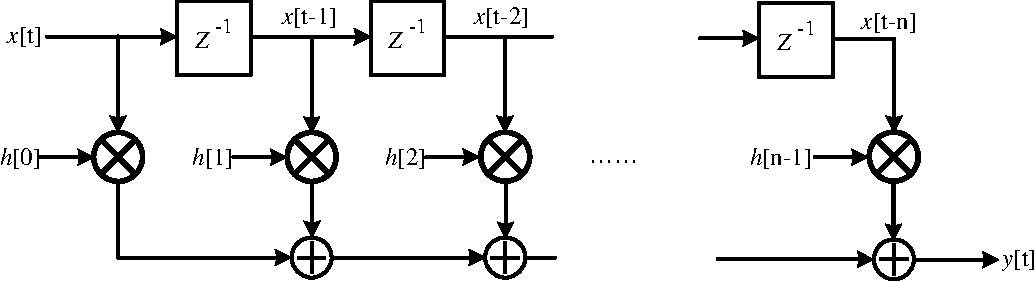
\includegraphics[width=\linewidth,height=0.52\textheight,keepaspectratio,alt={A typical FIR filter structure}]{md-to-tex-slides.figures/fir_strctr.pdf}
\caption{A typical FIR filter structure}
\end{figure}

\begin{itemize}
\tightlist
\item
  a converted figure can lose every label (\texttt{h{[}0{]}},
  \texttt{x{[}t-1{]}}, \texttt{y{[}t{]}}) 🏷️
\item
  a picture can look ``present'' yet be \textbf{informationally empty}
  🕳️
\end{itemize}
\end{frame}

\begin{frame}[fragile]{🧩 War Story 6: cleveref vs
\texttt{siamltex.cls}}
\protect\phantomsection\label{war-story-6-cleveref-vs-siamltex.cls}
\begin{center}
\begin{tikzpicture}[node distance=11mm and 14mm]
  \node[nblue] (cl) {cleveref hooks the\\label / counter machinery};
  \node[nred, right=of cl] (m) {\texttt{siamltex.cls}\\redefines them};
  \node[nred, right=of m] (e) {label type empty\\→ every ref is \texttt{??} ❌};
  \node[nyellow, below=10mm of cl] (fix) {\texttt{cref = false}\\§ + plain reference};
  \node[ngreen, right=16mm of fix] (ok) {§ 2, § 3.1 ✅};
  \draw[ar] (cl) -- (m);
  \draw[ar] (m) -- (e);
  \draw[ar] (fix) -- (ok);
\end{tikzpicture}
\end{center}

\begin{itemize}
\tightlist
\item
  proven with a \textbf{minimal test}: \texttt{article} + cleveref →
  fine; \texttt{siamltex} + cleveref → \texttt{??} 🔬
\item
  \textbf{latest pandoc} does not help --- it is the \textbf{class}, not
  the version 📌
\end{itemize}
\end{frame}

\begin{frame}[fragile]{📴 War Story 7: Citations That Phone Home}
\protect\phantomsection\label{war-story-7-citations-that-phone-home}
\begin{center}
\begin{tikzpicture}[node distance=9mm and 12mm]
  \node[nblue] (a) {\texttt{*.csl}\\dependent style};
  \node[nblue, right=of a] (b) {\texttt{independent-parent}\\= elsevier-with-titles};
  \node[nred, right=of b] (net) {🌐 fetch from\\zotero.org};
  \node[nred, right=of net] (fail) {ConnectionTimeout ❌};
  \node[nyellow, below=11mm of a] (inline) {inline the parent};
  \node[ngreen, right=of inline] (self) {self-contained ✅\\offline};
  \draw[ar] (a) -- (b);
  \draw[ar] (b) -- (net);
  \draw[ar] (net) -- (fail);
  \draw[ar] (inline) -- (self);
\end{tikzpicture}
\end{center}

\begin{itemize}
\tightlist
\item
  that CSL file was only a \textbf{stub} --- its citation / bibliography
  logic lived in a parent 🧩
\item
  every fresh machine / CI fetches it → flaky and
  \textbf{non-reproducible} 🎲
\item
  fix: \textbf{vendor the parent} → \texttt{-\/-citeproc} works
  \textbf{offline} (verified with a dead proxy) 🔒
\end{itemize}
\end{frame}

\section{Engineering the Build}\label{engineering-the-build}

\begin{frame}[fragile]{⚙️ One Entry Point: the \texttt{Makefile}}
\protect\phantomsection\label{one-entry-point-the-makefile}
{\def\LTcaptype{none} % do not increment counter
\begin{longtable}[]{@{}ll@{}}
\toprule\noalign{}
target & produces \\
\midrule\noalign{}
\endhead
\texttt{make\ paper} & \texttt{ell-review.pdf} 📕 \\
\texttt{make\ html} & \texttt{ell-review.html} (needs \texttt{katex/})
🌐 \\
\texttt{make\ slides} & \texttt{cutting\_plane.pdf}, \texttt{ell.pdf}
(xelatex) 🖥️ \\
\texttt{make\ clean} & remove \texttt{temp.*} and aux files 🧹 \\
\bottomrule\noalign{}
\end{longtable}
}

\begin{Shaded}
\begin{Highlighting}[]
\NormalTok{paper: ell{-}review.pdf}

\NormalTok{ell{-}review.pdf: ell{-}review.md}
\NormalTok{    pandoc {-}F pandoc{-}crossref {-}{-}citeproc {-}s {-}t latex {-}N \textbackslash{}}
\NormalTok{      {-}{-}reference{-}links {-}{-}shift{-}heading{-}level{-}by={-}1 \textbackslash{}}
\NormalTok{      ell{-}review.yaml latex.yaml crossref.yaml ell{-}review.md {-}o $@}
\end{Highlighting}
\end{Shaded}

\begin{quote}
The \texttt{Makefile} records the \textbf{flags \emph{and} the reasons}
--- no more tribal knowledge. 📌
\end{quote}
\end{frame}

\begin{frame}[fragile]{🪟 Make on Windows: Two Gotchas}
\protect\phantomsection\label{make-on-windows-two-gotchas}
\begin{columns}[T]
\begin{column}{0.47\linewidth}
\textbf{1. Recipes are exec'd directly} 🐚

\begin{itemize}
\tightlist
\item
  a \emph{simple} recipe runs \textbf{without a shell}
\item
  \texttt{rm} is not an \texttt{.exe} here →
  \texttt{CreateProcess\ failed} ❌
\item
  force a shell with a metacharacter ✅
\end{itemize}

\begin{Shaded}
\begin{Highlighting}[]
\NormalTok{clean:}
\NormalTok{    {-}@rm {-}f temp.tex temp.pdf ; true}
\end{Highlighting}
\end{Shaded}
\end{column}

\begin{column}{0.47\linewidth}
\textbf{2. Line endings} 📏

\begin{itemize}
\tightlist
\item
  LF in the repo, CRLF on disk
\item
  keeps diffs \textbf{logical}, not whole-file 🔍
\end{itemize}

\textbf{3. Version-matched tools} ⚖️

\begin{itemize}
\tightlist
\item
  \texttt{pandoc} and \texttt{pandoc-crossref} must agree
\item
  a mismatch warns and can misbehave silently 🎭
\end{itemize}
\end{column}
\end{columns}
\end{frame}

\begin{frame}[fragile]{🧹 Repo Hygiene}
\protect\phantomsection\label{repo-hygiene}
\begin{itemize}
\tightlist
\item
  \textbf{editor backups} (\texttt{*\textasciitilde{}},
  \texttt{*.un\textasciitilde{}}) --- untrack and \texttt{.gitignore}
  them 🗑️
\item
  \textbf{stale outputs} (\texttt{ell-review.tex}, \texttt{main-diff.*})
  --- generated, not source 📜
\item
  \textbf{one self-contained CSL} --- no network at build time 📴
\item
  \textbf{one linter, one config} --- two disagreeing linters equal
  \emph{zero} linters 🎭
\item
  \textbf{refresh the agent guide} --- write the \emph{why} while it is
  fresh 🧠
\end{itemize}

\begin{center}
\begin{tikzpicture}[node distance=14mm and 26mm]
  \node[nblue] (a) {commit sources only};
  \node[nyellow, right=of a] (b) {artifacts generated,\\never hand-edited};
  \node[ngreen, right=of b] (c) {reproducible:\\any machine, offline ✅};
  \draw[ar] (a) -- (b);
  \draw[ar] (b) -- (c);
\end{tikzpicture}
\end{center}
\end{frame}

\begin{frame}[fragile]{🔍 Verify the Artifact, Not the Exit Code}
\protect\phantomsection\label{verify-the-artifact-not-the-exit-code}
\begin{Shaded}
\begin{Highlighting}[]
\FunctionTok{make}\NormalTok{ paper                                 }\CommentTok{\# exit 0 is necessary, not sufficient}
\ExtensionTok{pdfinfo}\NormalTok{ ell{-}review.pdf                     }\CommentTok{\# page count}
\ExtensionTok{pdftotext}\NormalTok{ ell{-}review.pdf }\AttributeTok{{-}} \KeywordTok{|} \FunctionTok{grep} \AttributeTok{{-}c} \StringTok{\textquotesingle{}??\textquotesingle{}}  \CommentTok{\# unresolved references}
\end{Highlighting}
\end{Shaded}

\begin{itemize}
\tightlist
\item
  \texttt{??} count → did the cross-references resolve? 🔗
\item
  extracted text → are the \textbf{figure labels} present? (catches
  dropped SVG text) 🏷️
\item
  page count → did the build actually \textbf{change} anything? 📄
\item
  a tiny \textbf{CI job} running \texttt{make\ paper} would have caught
  the stale PDF 🚨
\end{itemize}
\end{frame}

\begin{frame}[fragile]{✅ Reproducibility Checklist}
\protect\phantomsection\label{reproducibility-checklist}
\begin{columns}[T]
\begin{column}{0.47\linewidth}
\textbf{Dependencies} 📦

\begin{itemize}
\tightlist
\item
  pandoc \textbf{and} pandoc-crossref, version-matched ⚖️
\item
  a LaTeX engine (\texttt{pdflatex} / \texttt{xelatex}) 📐
\item
  an SVG converter \textbf{or} committed PDF twins 🖼️
\end{itemize}
\end{column}

\begin{column}{0.47\linewidth}
\textbf{Sources} 📝

\begin{itemize}
\tightlist
\item
  a self-contained CSL (offline) 📴
\item
  ASCII math, no emoji (or xelatex) 🔤
\item
  exactly one crossref policy ⚙️
\end{itemize}
\end{column}
\end{columns}

\begin{center}
\begin{tikzpicture}[node distance=14mm and 26mm]
  \node[nblue] (a) {same inputs};
  \node[nyellow, right=of a] (b) {same command};
  \node[ngreen, right=of b] (c) {same output ✅};
  \draw[ar] (a) -- (b);
  \draw[ar] (b) -- (c);
\end{tikzpicture}
\end{center}
\end{frame}

\begin{frame}[fragile]{🎯 Key Takeaways}
\protect\phantomsection\label{key-takeaways}
\begin{columns}[T]
\begin{column}{0.47\linewidth}
\textbf{The pipeline} 🏭

\begin{itemize}
\tightlist
\item
  pandoc + crossref + citeproc turns Markdown into journal-ready TeX 📕
\item
  one \texttt{make} target beats a notebook of shell history 📓
\end{itemize}

\textbf{The habit} 🧠

\begin{itemize}
\tightlist
\item
  inspect the \textbf{artifact}, not the exit code 🔍
\item
  vendor \textbf{everything} remote --- a build must work offline 📴
\end{itemize}
\end{column}

\begin{column}{0.47\linewidth}
\textbf{The traps} 🪤

\begin{itemize}
\tightlist
\item
  non-ASCII (emoji, bare Unicode) kills \texttt{pdflatex} ☠️
\item
  old classes can break cleveref → every reference becomes \texttt{??}
  🧩
\item
  ``standard-looking'' macros may not exist
  (\texttt{\textbackslash{}argmax}) 🐛
\end{itemize}
\end{column}
\end{columns}
\end{frame}

\begin{frame}[fragile]{📚 References \& Further Reading}
\protect\phantomsection\label{references-further-reading}
\begin{itemize}
\tightlist
\item
  \textbf{pandoc} --- the user's guide \& MANUAL:
  \url{https://pandoc.org/MANUAL.html} 📖
\item
  \textbf{pandoc-crossref} --- labels for sections, figures, equations
  🔗
\item
  \textbf{CSL --- Citation Style Language}:
  \url{https://citationstyles.org} 🎨
\item
  \textbf{cleveref} --- and why older document classes can fight it 🧩
\item
  the paper: \textbf{``Ellipsoid Method and the Amazing Oracles''} 📕
\end{itemize}

\begin{quote}
Assembled for the \texttt{ellipsoid-method} repo; the full checklist
lives in \textbf{issue \#4}. 🗂️
\end{quote}
\end{frame}

\begin{frame}{🙋 Q\&A}
\protect\phantomsection\label{qa}
\textbf{From Markdown to TeX --- A Pandoc Paper Pipeline}

Questions? Discussion? 💬
\end{frame}

\begin{frame}{👏 Thank You}
\protect\phantomsection\label{thank-you}
Same input, same command, same output. 🎯

Slides built with Beamer · TikZ 🧩 · LuaLaTeX 📐 · Nord 🌙
\end{frame}

\end{document}
